\chapter{Creating an Adventurer}
To play in \textbf{Adventure Quest} (\textbf{AQ} for short), you must first create an adventurer to control during the game. All adventurers start out as young persons just leaving home, seeking fame, fortune and yet more adventure. Keep track of your adventurer's attributes and skills by completing an adventurer card The one below is designed to fit on a 4x6 notecard. If you'd like one that expands a bit more and takes up a full sheet of paper, you can find an example in \appage{ap:adventurer-record-full}. Use a pencil for this, as frequent changes will be made during the adventurer's career.

\begin{tabularx}{\linewidth}{@{\extracolsep{\fill}} l l l l l l l l }
\midrule
Name: & & & ( & & \makecell[r]{)} & Rate & \\
STR & & Background & & & Mod / Defense & Date & \\
INT & & DP & & Combat & \makecell[c]{/} & Silver & \\
PER & & EU/DU & & Missile & \makecell[c]{/} & EXP & \\
CSE & & Element & & Grapple & \makecell[c]{/} & Profession & \\
HEA & & Languages: & & Skills: & Equipment: & Enchanted Items: & \\
AGI & & & & & & & \\
PWR & & & & & & & \\
COM & & & & & & & \\
WIL & & & & & & & \\
& & & & & & & \\
Race & & & & & & & \\
Sex & & & & & & & \\
DoB & & & & & & & \\
Age & & & & & & & \\
Build & & & & & & & \\
Height & & & & & & & \\
Weight & & & & & & & \\
Eye & & & & & & & \\
Hair & & & & & & & \\
Motive & & & & & & & \\
Deity & & & & & & & \\
\midrule\end{tabularx}\smallskip
%\setlength{\columnsep}{\defcolwidth}\begin{multicols*}{2}

When people are born, they do not get to choose to be male or female, tall or short, or clever or daft. To simulate this in AQ, these attributes (and other uncontrollable random events) are determined by rolling dice. Later, you may freely choose the skills, languages, etc. your adventurer learns as they grow. 
\section{Physical Statistics}

Each adventurer has several attributes. The most important of these are the nine physical statistics or stats, which are listed at the top of the first column of the adventurer card. These stats normally have a rank or value between 0 and 24.

\noindent\begin{normbox}[Physical Statistics]
\small
\begin{tabular}{@{}l l}
Strength (STR) & Physical prowess\\
Intelligence (INT) & Reasoning and problem solving\\
Perception (PER) & Awareness of surrounding events\\
Common Sense (CSE) & Sound practical judgement\\
Health (HEA) & Physical well-being\\
Agility (AGI) & Physical coordination\\
Power  (PWR) &  Magical potential\\
Comeliness (COM) & Physical beauty\\
Willpower (WIL) & Mental strength\\
\end{tabular}
\normalsize
\end{normbox}

Each stat is generated by totaling the roll of 3d6, and thus ranges from 3 to 18. Roll 3d6 and write the total opposite STR on the card , roll again and write the total opposite INT, etc. until all stats have a value. Do not despair if they are not all high; playing an adventurer with both strong and weak points is much more fun and interesting than playing an omnipotent adventurer who never needs to think.
\section{Placed Roll}
After rolling the stats, you may change them somewhat to fit the kind of adventurer you wish to play. Roll 4d6 and throw any one die out, totaling the remaining three. Use this total to replace the value of any of your nine original stats. If the roll is unsatisfactory, ignore it and leave your stats unchanged.
\section{Life Force}
All adventurers have a Life Force, which starts equal to the total of their HEA and PER stats, but can be improved separately to those skills. For now, simply note the LF value on your adventurer's record.
\section{Race}

%\begin{wrapfigure}[9]{l}[0pt]{85pt}
\begin{normbox}[Race Roll]
\small
\begin{tabular}{@{}l l}
\textbf{Roll} & \textbf{Race}\\
\midrule
01 - 14 & Human\\
15 & Elf\\
16 & Dwarf \\
17 & Lizard\\
18 & Orc\\
19 - 20 & Half-breed
\end{tabular}
\end{normbox}\smallskip
%\end{wrapfigure}

Your adventurer may be one of five different races of intelligent creatures. Members of different races have differing physical appearances and abilities; see \chpage{ch:jaern-humanoids}. Roll 1d20 and check on the Race Roll table to determine your adventurer's race.

If the roll is 19 or 20, this means the adventurer's parents were of different races. Now roll to find the race of each parent. Each must be a different race, of course, so if the second parent roll is the same as the first, roll again until a different race is determined. The parents may be half-breeds themselves, which means that the adventurer's grandparents must be determined the same way. If a half-breed grandparent is rolled, ignore it and roll again. Racial heritage determines which racial skills your adventurer has. 

\begin{normbox}[Racial Traits]
\small
\begin{tabular}{l}
\makecell[l]{\textbf{Elf}\\
\midrule
1. Exceptional PER\\
2. Distance Judgment\\
3. Missile Skill*\\
4. Soulless }\\ 
\makecell[l]{\textbf{Orc}\\
\midrule
1. Exceptional WIL\\
2. Enhanced Smell\\
3. Physical Viciousness*\\
4. Mental Stubbornness}\\
\makecell[l]{\textbf{Dwarf}\\
\midrule
1. Exceptional HEA\\
2. Material Sense\\
3. Armor Construction*\\
4. Great Durability }\\
\makecell[l]{\textbf{Lizard}\\
\midrule
1. Exceptional AGI\\
2. Quickness\\
3. Water Breathing\\
4. Homing}\\
\end{tabular}
\end{normbox}
*See \chref{ch:jaern-humanoids} to learn about these skills.
\normalsize

Non-physical differences are represented as racial skills. For each list below in which your adventurer has a grandparent, roll 1d4 for each skill. If the number is equal to or less than the number of grandparents of that race, write that skill on the adventurer card. If your adventurer is purebred, (i.e. all four grandparents are the same race) they automatically get all that race's skills. Read the \chref{ch:jaern-humanoids} to learn about these skills and racial disadvantages.

Elves are extremely long lived compared to the other races. They do not, however, posses a soul, and thus do not have an existence after death. This makes then unable to use divine magic, and unable to ever be brought back from the dead. Elves generally do not interact with the deities and their priests. Holy places like temples and shrines make them feel uncomfortable and they tend to avoid them.

Full Humans are often more diverse and adaptable than other races. If your adventurer is a full bred human, you may take an additional Placed Roll to further customize your stats. Roll 4d6 and throw any one die out, totaling the remaining three. Use this total to again replace the value of any of your nine original stats. If the roll is unsatisfactory, ignore it and leave your stats unchanged.
\section{Sex}


%\begin{wrapfigure}[5]{l}[0pt]{60pt}
\begin{normbox}[Sex Roll]

\small
\begin{tabular}{@{}l l}
\textbf{Roll} & \textbf{Sex}\\
\midrule
1-3 & Male\\
4-6 & Female
\end{tabular}
\end{normbox}
%\end{wrapfigure}

Choose a sex for your adventurer, or roll 1d6 and check against the following table. You may additionally choose to play an intersex character, and your character may present as any gender of their choice.
\section{Age}


%\begin{wrapfigure}[6]{l}[0pt]{60pt}
\begin{normbox}{Age Die}
\small

\begin{tabular}{@{}l l}
\textbf{Race} & \textbf{Die}\\
\midrule
Orc & d4\\
Human & d6\\
Lizards &  d8\\
Dwarf & d10\\
Elf &  d20\\
\end{tabular}
\normalsize
\end{normbox}
%\end{wrapfigure}

Determine how old your adventurer is at the start of his or her career by rolling one die of the appropriate type for each grandparent, and add +10 to the result. Aging is covered in detail in \chpage{ch:jaern-humanoids}.

If your adventurer is pure human, obviously all four of their grandparents are human. Roll 4d6, total them and add +10 to find out their age.

If, for example, they are half-elf, quarter-human and quarter-dwarf, roll 2d20 + 1d6 + 1d10 + 10.

\section{Body build}

If your adventurer is not purebred, roll 1d4 to randomly select a grandparent' s race, then roll 1d20 to determine your adventurer's body build using the appropriate race on the following table. If your adventurer is female, her body build is one category smaller than the chart result.
\begin{normbox}[Body Build]
\small
\begin{tabular}{@{} l l l l l l }
 & \textbf{Orc} & \textbf{Elf} & \textbf{Human} & \textbf{Dwarf} & \textbf{Lizard}\\
\midrule
A & - & - & - & - & -\\
B & 1 & 1-2 & - & - & -\\
C & 2-5 & 3-6 & 1-2 & - & -\\
D & 6-16 & 7-14 & 3-6 & 1 & 1-2\\
E & 17-19 & 15-18 & 7-14 & 2-5 & 3-6\\
F & 20 & 19-20 & 15-18 & 6-16 & 7-14\\
G & - & - & 19-20 & 17-19 & 15-18\\
H & - & - & - & 20 & 19-20
\end{tabular}
\end{normbox}

\section{Height and Weight}

%\begin{wrapfigure}[7]{l}[0pt]{60pt}
\begin{normbox}[Racial Height]
\small

\begin{tabular}{@{}l l}
Dwarves & +0\\
Orcs & +2\\
Humans & +4\\
Elves & +5\\
Lizards & +6\\
\end{tabular}
\end{normbox}
%\end{wrapfigure}

\normalsize
Height and weight are determined by rolling 4d6 and totaling them. Add the number shown below for the race of each grandparent. Now look up the resulting number on the following table, referencing the number to the appropriate body build column:

\begin{normbox}[Height and Weight]
\begin{tabularx}{\linewidth}{@{} X X X X X X X X X X | X X X X X X X X X X}
\small
\textbf{\#} & \textbf{HGT} & \textbf{A} & \textbf{B} & \textbf{C} & \textbf{D} & \textbf{E} & \textbf{F} & \textbf{G} & \textbf{H} & \textbf{\#} & \textbf{HGT} & \textbf{A} & \textbf{B} & \textbf{C} & \textbf{D} & \textbf{E} & \textbf{F} & \textbf{G} & \textbf{H}\\
%\midrule
4 & 3'7" & 29 & 35 & 42 & 51 & 62 & 74 & 89 & 108 & 27 & 5'6" & 70 & 85 & 102 & 123 & 148 & 179 & 215 & 259\\
5 & 3'8" & 31 & 37 & 44 & 54 & 65 & 78 & 94 & 113 & 28 & 5'7" & 73 & 88 & 105 & 127 & 153 & 184 & 222 & 268\\
6 & 3'9" & 32 & 39 & 47 & 56 & 68 & 81 & 98 & 118 & 29 & 5'8" & 75 & 90 & 109 & 131 & 158 & 190 & 229 & 276\\
7 & 3'10" & 34 & 40 & 49 & 59 & 71 & 85 & 103 & 124 & 30 & 5'9" & 77 & 93 & 112 & 135 & 163 & 196 & 236 & 285\\
8 & 3'11" & 35 & 42 & 51 & 61 & 74 & 89 & 107 & 129 & 31 & 5'10" & 80 & 96 & 115 & 139 & 168 & 202 & 243 & 293\\
9 & 4'0" & 37 & 44 & 53 & 64 & 77 & 93 & 112 & 135 & 32 & 5'11" & 82 & 99 & 119 & 143 & 173 & 208 & 251 & 302\\
10 & 4'1" & 38 & 46 & 55 & 67 & 80 & 97 & 117 & 141 & 33 & 6'0" & 84 & 102 & 122 & 148 & 178 & 214 & 258 & 311\\
11 & 4'2" & 40 & 48 & 58 & 70 & 84 & 101 & 122 & 146 & 34 & 6'1" & 87 & 105 & 126 & 152 & 183 & 220 & 266 & 320\\
12 & 4'3" & 41 & 50 & 60 & 72 & 87 & 105 & 127 & 153 & 35 & 6'2" & 89 & 108 & 130 & 156 & 188 & 227 & 273 & 329\\
13 & 4'4" & 43 & 52 & 63 & 75 & 91 & 109 & 132 & 159 & 36 & 6'3" & 92 & 111 & 133 & 161 & 194 & 233 & 281 & 339\\
14 & 4'5" & 45 & 54 & 65 & 78 & 94 & 114 & 137 & 165 & 37 & 6'4" & 94 & 114 & 137 & 165 & 199 & 240 & 289 & 348\\
15 & 4'6" & 47 & 56 & 68 & 81 & 98 & 118 & 142 & 171 & 38 & 6'5" & 97 & 117 & 141 & 170 & 205 & 246 & 297 & 358\\
16 & 4'7" & 48 & 58 & 70 & 85 & 102 & 123 & 148 & 178 & 39 & 6'6" & 100 & 120 & 145 & 174 & 210 & 253 & 305 & 368\\
17 & 4'8" & 50 & 60 & 73 & 88 & 106 & 127 & 153 & 185 & 40 & 6'7" & 102 & 123 & 149 & 179 & 216 & 260 & 313 & 377\\
18 & 4'9" & 52 & 63 & 75 & 91 & 110 & 132 & 159 & 192 & 41 & 6'8" & 105 & 127 & 153 & 184 & 222 & 267 & 322 & 388\\
19 & 4'10" & 54 & 65 & 78 & 94 & 114 & 137 & 165 & 199 & 42 & 6'9" & 108 & 130 & 157 & 189 & 227 & 274 & 330 & 398\\
20 & 4'11" & 56 & 67 & 81 & 98 & 118 & 142 & 171 & 206 & 43 & 6'10" & 111 & 133 & 161 & 194 & 233 & 281 & 339 & 408\\
21 & 5'0" & 58 & 70 & 84 & 101 & 122 & 147 & 177 & 213 & 44 & 6'11" & 114 & 137 & 165 & 199 & 239 & 288 & 348 & 419\\
22 & 5'1" & 60 & 72 & 87 & 105 & 126 & 152 & 183 & 220 & 45 & 7'0" & 117 & 140 & 169 & 204 & 246 & 296 & 356 & 429\\
23 & 5'2" & 62 & 75 & 90 & 108 & 130 & 157 & 189 & 228 & 46 & 7'1" & 119 & 144 & 173 & 209 & 252 & 303 & 365 & 440\\
24 & 5'3" & 64 & 77 & 93 & 112 & 135 & 162 & 196 & 236 & 47 & 7'2" & 122 & 148 & 178 & 214 & 258 & 311 & 374 & 451\\
25 & 5'4" & 66 & 80 & 96 & 116 & 139 & 168 & 202 & 243 & 48 & 7'3" & 125 & 151 & 182 & 219 & 264 & 318 & 384 & 462\\
26 & 5'5" & 68 & 82 & 99 & 119 & 144 & 173 & 209 & 251 & 									
\end{tabularx}
\end{normbox}

%\begin{tcbraster}[raster columns=1,boxrule=0pt,title=\small\textbf{Height and Weight Table},left=0pt,right=0pt,top=0pt,bottom=0pt,boxsep=0pt,boxrule=0.6pt,lefttitle=2.5mm,toptitle=1mm,bottomtitle=1mm,colbacktitle=Navy,colback=white]

%\tcbincludepdf{height-weight-vertical.pdf}
%\end{tcbraster}
%\end{normbox}
%\begin{multicols*}{2}
\normalsize
\section{Eye color}

If your adventurer is not purebred, roll 1d4 to randomly select a grandparent's race. Roll 1d20 to find your adventurer's eye color.

\begin{normbox}[Eye Color]
\small
\begin{tabular}{@{}l l l l l l}
\textbf{Color} & \textbf{Human} & \textbf{Elf} & \textbf{Dwarf} & \textbf{Orc} & \textbf{Lizard}\\
\midrule
Black & 1 & 1-2 & 1-10 & 1-4 & 1-12\\
Brown & 2-8 & -- & 11-18 & 5-6 & --\\
Blue & 9-14 & 3-10 & -- & -- & 13-15\\
Green & 15-16 & 11-14 & 19-20 & 7-12 & 16\\
Red & -- & 15-17 & -- & 13-18 & 17-19\\
Silver & -- & 18-19 & -- & -- & 20\\
Hazel & 17-20 & -- & -- & 19-20 & --\\
White & -- & 20 & -- & -- & --
\end{tabular}
\end{normbox}
\section{Hair color}


If your adventurer is not purebred, roll 1d4 to randomly select a grandparent's race. Now roll 1d20 to find your adventurer's hair color, using the appropriate race column on this table:

\begin{normbox}[Hair Color]
\small
\begin{tabular}{@{}l l l l l l}
\textbf{Color} & \textbf{Human} & \textbf{Elf} & \textbf{Dwarf} & \textbf{Orc} & \textbf{Lizard}\\
\midrule

Brown & 1-7 & -- & 1-10 & 1-2 & --\\
Black & 8-11 & 1-6 & 11-16 & 3-16 & --\\
Blond & 12-15 & 7-8 & -- & -- & --\\
Red & 16-17 & 9-13 & 17 & 17-18 & --\\
Green & -- & 14-15 & -- & 19 & --\\
Grey & 18 & -- & 18 & -- & --\\
White & 19 & 16-18 & -- & 20 & --\\
None & 20 & -- & 19-20 & -- & 1-20\\
Silver & -- & 19-20 & -- & -- & --
\end{tabular}
\end{normbox}
\section{Motivation}
That takes care of the random elements of adventurer creation; now you have a free hand in developing your adventurer's inner-self. Evolving his personality takes some thought, but it is a rewarding aspect of role-playing. A good way to start is to create an event that occurred early in his life that now defines his basic motivation. Once you have a starting point it is easier to describe more about their personality.

Below are some possible motivations from which to choose, but you are free to make up others as best fits your needs and concepts. Now mentally describe an event or condition to explain why it is your adventurer's primary motivation. Write this motive down on the Adventurer Card after "Motive." Here are some suggestions:

\begin{normbox}[Motivation]
\small
\begin{tabularx}{\linewidth}{@{} l L}
Duty & Allegiance to a higher authority\\
Fame & Gaining recognition from others\\
Justice & Maintaining balance\\
Knowledge & Learning for learning's sake\\
Passion & Serving a cause with intense emotional fervor\\
Pleasure & Seeking pleasures of the flesh\\
Power & Forcing the submission of others\\
Religion & Devoting their life to a higher authority\\
Righteousness & Striving to help mankind\\
Romance & Earning the love and/or respect of others
\end{tabularx}
\end{normbox}

The motive you choose is not meant to be a "straight jacket" to force you to play the adventurer within narrow bounds. It is meant to be used, by you, to help set a direction for your adventurer's actions and a start for his personality. You always have the freedom to write down what you believe is your adventurer's driving force on your card. Also realize that there is magic which can be used to determine your motive, and the results of this magic will be what is perceived by the GM as your motive, which may disagree with what you have written.
To learn more about creating your adventurer's personality, read \chref{ch:creating-actors} to see how the GM creates personalities for actors. These methods are applicable to your adventurer's personality as well.
\section{Patron Gods}

You may select one deity as your adventurer's patron god. Adventurers aligning themselves to a deity this way are expected to assist the causes of the god, and especially to follow that god's precepts and laws. In return, they are often assisted by the priests and followers of that deity. Worshiping more than one god is possible, but can become difficult if the deities conflict in any way. Write down the name(s) of the deity(s) on the adventurer card after "Deity." Here is a list of available deities; each is covered in detail in its own chapter.

\begin{normbox}[Patron Gods]
\small
\begin{tabular}{@{}l l l}

\textbf{God} & \textbf{Sphere of Influence} & \textbf{Chapter}\\
Ra & Bearer of Light & \ref{ch:ra}\\
Isis\ & Mistress of Life & \ref{ch:isis}\\
T'or\ & The Thunder of Righteousness & \ref{ch:t'or}\\
At'ena\ & Mistress of Wisdom & \ref{ch:at'ena}\\
Osiris\ & Protector of Nature & \ref{ch:osiris}\\
Tarus\ & Master Archivist & \ref{ch:tarus}\\
Neptune\ & Dweller of the Waters & \ref{ch:neptune}\\
Orus\ & The Flame of Zeal & \ref{ch:orus}\\
Anubis\ & Lord of the Dead & \ref{ch:anubis}\\
Rudri\ & Dweller of the Dark & \ref{ch:rudri}\\
Scrogg\ & Earthly Pleasures & \ref{ch:scrogg}\\
\end{tabular}
\end{normbox}
\normalsize

\section{Adventurer Background}
Backgrounds are the adventuring professions available in a specific AQ Game. Each Game has at least three major, divergent disciplines that may be followed, and thus gives three professions. Others are derived by combining two of the major disciplines to yield another, unique background. It may be helpful for you to visualize this as a three-spoke wheel, each spoke labeled with a major discipline. In AQ/Jaern these are Combat, Magic, and Skills.

\begin{center}

\tikzset{every picture/.style={line width=0.75pt}} %set default line width to 0.75pt        

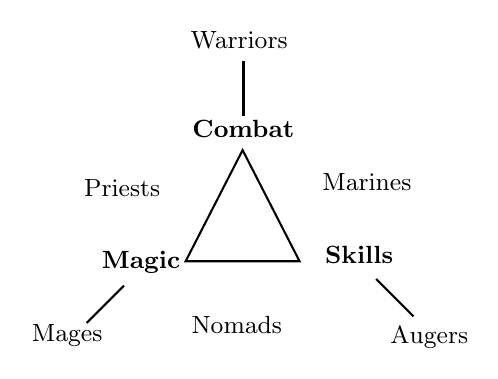
\begin{tikzpicture}[x=0.75pt,y=0.75pt,yscale=-0.9,xscale=0.9]
%uncomment if require: \path (0,300); %set diagram left start at 0, and has height of 300

%Straight Lines [id:da5792073549069615] 
\draw    (321.5,53) -- (321.5,82) ;
%Shape: Triangle [id:dp9921269194788708] 
\draw   (321,100.5) -- (351.5,160) -- (290.5,160) -- cycle ;
%Straight Lines [id:da10414083526965556] 
\draw    (257.5,173) -- (237.5,193) ;
%Straight Lines [id:da8045071749370871] 
\draw    (392.5,169.5) -- (412.5,189.5) ;

% Text Node
\draw (291.5,35.5) node [anchor=north west][inner sep=0.75pt]   [align=left] {\small Warriors};
% Text Node
\draw (234.5,114.5) node [anchor=north west][inner sep=0.75pt]   [align=left] {\small Priests};
% Text Node
\draw (362,111.5) node [anchor=north west][inner sep=0.75pt]   [align=left] {\small Marines};
% Text Node
\draw (206.5,192) node [anchor=north west][inner sep=0.75pt]   [align=left] {\small Mages};
% Text Node
\draw (292,187.5) node [anchor=north west][inner sep=0.75pt]   [align=left] {\small Nomads};
% Text Node
\draw (398.5,193.5) node [anchor=north west][inner sep=0.75pt]   [align=left] {\small Augers};
% Text Node
\draw (363.5,150.5) node [anchor=north west][inner sep=0.75pt]   [align=left] {\small \textbf{Skills}};
% Text Node
\draw (244,153) node [anchor=north west][inner sep=0.75pt]   [align=left] {\small \textbf{Magic}};
% Text Node
\draw (292.5,83) node [anchor=north west][inner sep=0.75pt]   [align=left] {\small \textbf{Combat}};


\end{tikzpicture}
\end{center}

The three backgrounds at the ends of the spokes are thus Warrior (for those exclusively trained in combat), Mages (magic), and Augers (skills). As for the areas between the spokes, a background that combines magic and combat produces the Priest, someone with a knowledge of magic and the physical training to back it up. Combining magic and skills yields a Nomad, with training in the mystical arts as well as skills. And finally, mixing combat and skills produces a Marine, a person with a need for fighting ability and quick and nimble movements.

\begin{normbox}[Adventurer Background Stats]

\small
\begin{tabular}{@{}l l}
\textbf{Adventurer Background} & \textbf{Most Important Stat}\\
\midrule
Warrior & CSE and STR\\
Priest &  PWR and CSE\\
Magician &  PWR and INT\\
Nomad &  PER and HEA\\
Auger &  INT and CSE\\
Marine &  AGI and STR
\end{tabular}
\end{normbox}

Each background has one or more stats that is very important to the successful practice of the profession, as given in the above table. If your adventurer's highest stat is
STR, they probably would fare best as a Warrior. If they have a high PER, you probably should consider making them a Nomad, etc.

You must now choose an available background for your adventurer. Consider not only the stats, but also what you envision your persona becoming, or what you want to roleplay. You are not forced to pick the background that matches the highest stat. In fact, successfully role-playing (for example) an adventurer with a high STR and a mediocre INT as a Auger rather than a Warrior is very rewarding, not to mention entertaining, to you, the GM, and other players.Here are descriptions of the available backgrounds to further help you make a selection:\begin{itemize}
\item {A Warrior relies upon their skill at arms. They are proficient at fighting and confident in their ability to succeed with force. While they might serve in an army, a warrior prefers individual combat and is more likely found employed as a bodyguard, mercenary, constable, or a guard.}

\item A Priest is devoted to the service of a deity, forever at that deity's disposal to spread their faith and worship throughout the world. A priest is willing for fight for their deity's cause, but can also use god-given magical powers to further their goals.

\item A Magician is a practitioner of one of four types of elemental magics, using his magics to affect the world and gain wealth, recognition and influence. A magician is often consulted and employed by others to accomplish their goals.
The spells available in each element give a definite flavor to the personality and style of play of a magician. Fire and Air magicians tend to have more offensive spells, whereas Earth and Water mages are more defense oriented. Fire and Earth magic tends to be more individual in nature, while many Air and Water spells are useful to support and maintain a group of adventurers. If your adventurer is going to become a magician, bear these generalities in mind to select the elemental style that matches your adventurer's personality.

\item Brought up learning to think to solve their problems, an Auger's basic tenet is to live up to their potential, learning to utilize their best skills and making the most of any situation.
\item Born to the seas, a Marine is a member of the traveling armies that plies the seas of Jaern. Ready with a quick story of marine heroes of the past, today's marine attempts to make a name for themselves and their shipmates. They adventure for fame, and are always ready for a good fight and a large tankard of ale.

\item Members of a tight-knit group of families, Nomads mistrust all other Jaernians and rarely travel among them. They are rumored to have various mystical and magical powers, so most people shun them, unsure of their intentions.
\end{itemize}
After choosing one of these, place it on the adventurer card after "Background." If you're still uncertain, scan the list of Model Adventurers beginning on \tcpage{create-models} for ideas and suggestions. If it appears your adventurer suffers from hopelessly inadequate stats, they would probably not become an adventurer in a fantasy world. Ask the GM; they may allow you to discard this would-be adventurer and start over.
\section{Languages}
You need to know which languages (if any) your adventurer speaks to know how they can communicate with actors and other adventurers. Knowledge of languages is an intelligence-based skill, and beginning adventurers may know zero, one or two languages.


%\begin{wrapfigure}[11]{l}[0pt]{4cm}
\begin{normbox}[Learned Language]
\label{create-language}
\small
\begin{tabular}{l l l}
INT & \makecell{Initial\#} & \makecell{Max\#}\\
\midrule
3 - 5 & 0 & 0\\
6 - 8 & 1 & 1\\
9 - 11 & 2 & 2\\
12 - 14 & 2 & 3\\
15 - 17 & 2 & 4\\
18 - 20 & 2 & 5\\
21 - 23 & 2 & 6\\
24+ & 2 & 7\\
\end{tabular}
\normalsize
\end{normbox}
%\end{wrapfigure}

Adventurers having less than INT 6 cannot speak coherently. They may know how to say isolated words or phrases, and can generally understand simple sentences. Playing adventurers with a low INT is very challenging because the player must communicate through actions rather than words.

The first language an adventurer with greater than INT 6 learns is their racial language. This is Paroli for all human adventurers. Half-breed adventurers may pick one of their racial languages as their native tongue or the tongue of whomever raised them, whichever is most appropriate. The first language is always known at a skill rank 9 or the adventurer's INT, whichever is lower.

Above INT 8, the player may choose a second language. For non-human adventurers, it would be prudent to pick the common tongue of the area to simplify communications. This second language is initially known at a skill rank 6.

\begin{normbox}[Languages]

\small
\begin{tabularx}{\linewidth}{@{} l X }
Breziak & Human tongue\\
Dwarvish & Race tongue of dwarves\\
Elvish & Race tongue of most elves\\
Entish & Spoken by intelligent forest creatures\\
Ferric & Human tongue\\
Geleik & Tongue of the elves of Silvan Isle\\
Haoogh & Speech of the southern pirates\\
Orcish & Race tongue of orcs\\
Paroli & Race tongue for humans and common tongue\\
Sel'ict & Race tongue of the lizard men\\
Trejon & Ancient human tongue\\
\end{tabularx}
\normalsize
\end{normbox}
\setlength{\columnsep}{0.25cm}
\section{Rating}
Your GM must be able to balance your adventuring party against some opponents it might meet. Your adventurer's Rating is how many adventurers they have experienced. Set this at two now, and each time he finishes a gaming session, add one. A starting rating of two represents the skills that you choose in creating your adventurer. Your GM may ask for this number from all the players at the beginning of a gaming session.
\section{Date}

At the beginning and end of each adventure, the Game Master will tell you the current game date. The amount of time elapsed between adventures is important for curing damage, doing research, being pregnant, etc. The date is in ISO 8601 format (Year-Month-Day), such as 10080-06-15 SF (Since Founding). Record the current date minus your age on your card as your date of birth (DOB).
\section{Nomadic Prefix Names}


%\begin{wrapfigure}[9]{l}[0pt]{5cm}
\begin{normbox}[Nomad Prefix Names]
\small
\begin{tabular}{l l|l l}
Roll & Prefix & Roll & Prefix\\
\midrule
1-5 & Raz- & 16 & Ald-\\
6-9 & Car- & 17 & Edo-\\
10-12 & Oka- & 18 & Ijo-\\
13-14 & Vem- & 19 & Bez-\\
15 & Lar- & 20 & Sag-\\
\end{tabular}
\normalsize
\end{normbox}
%\end{wrapfigure}

If your adventurer is a Nomad, then they must know their own prefix name, or Epokonom. Roll 1d20 and look at the following table. Put this prefix before your adventurer's name on your adventurer card.

\section{Name}
Each adventurer must have a name of some sort. Choose a name for your adventurer and place it in the upper left-hand corner of the card. After this put your real name in parenthesis. This will help the Game Master to remember whose adventurer is whose.
\section{Profession}
Your adventurer may have a regular job to bring in a steady income. After your adventurer's skills are selected (see \tcpage{create-skills}), you may choose one as their profession.
\pagebreak
\section{Adventurer Models}
Players buy attributes for their adventurers using experience points. Physical equipment is bought with silver pieces. This buying allows you to make your adventurer's abilities fit your perception of her personality.

To simplify making a new adventurer, several different Model Adventurers are reproduced here. If you wish to pick one of these, just copy the information from the chosen model that matches your adventurer's background onto an adventurer card. For each defense value listed in the model, plug in the appropriate stats from your adventurer (dividing them by 5 and rounding down as shown) and add the results to find the your adventurer's defense values. If they are an elf, add +1 on their \DV for Exceptional PER. If they are an orc, add +1 to their GDV for Exceptional WIL. Your adventurer is ready to play.

Each model allows you 20\% more attributes than if you had bought all the attributes separately. This extra does not make the adventurer more powerful; it is used to buy attributes that give added flavor and a direction for further development. Once selected, models cannot be modified or changed except to buy new attributes (or upgrade current ones) with earned experience points (see \chpage{create-buying}).

If none of the models fit your idea of your adventurer's personality, and your GM is allowing custom adventurer creation, skip this section and read to complete your adventurer's creation.

Each adventurer prototype specifies the values for the following attributes:

\begin{normbox}[Model Attributes]
\small
\noindent\begin{tabularx}{\columnwidth}{@{} l X}
Damage Points (\DP) & Relative health\\
Combat Modifier (\CM) & Ability using hand-to-hand weapons\\
Missile Modifier (\MM) & Ability using bows, slings and crossbows\\
Grapple Modifier (\GM) & Ability to grapple\\
Spell type & Declared type of spells (Earth, Fire, Aair, Water, and Divine)\\
Spell Groups & Ability to use various spell groups\\
Incants & Specific nomadic items and talisman\\
Skills & Purchased skills and their ranks\\
Combat Defense (CDV) & Resistance to being struck\\
Missile Defense (MDV) & Resistance to being hit by missiles\\
Grapple Defense (GDV) & Resistance to being grappled\\
\end{tabularx}
\end{normbox}
%\vfill\null\columnbreak
\subsection{Models}
\label{create-models}
TBD
\pagebreak
\section{Experience Points}
Experience Points (\EP) are the currency used to buy such attributes as skills, stats, spells groups, damage points, and melee modifiers. Your adventurer is awarded \EP during and after an adventure in several ways, depending on the method chosen by your GM. Using experience points in this way simulates any training or study that might be required to acquire or improve an ability without actually going through the tedium and boredom of doing so during a gaming session. By the way, when an adventure ends, don't forget to add +1 to the Rating entry on the adventurer's card. Your GM uses the rating to get a rough idea of how much experience your adventurer has had so that they may balance the difficulty of an adventure against the power of the adventurers.

You may specify that a portion of the awarded experience be set aside and used later to buy attributes. There is no limit to the amount of experience your adventurer may hold, but it makes little sense to hold it longer than needed to buy the attributes sought.
\section{Buying}
\label{create-buying}
If you have not chosen an Adventurer Model, your adventurer is given 5000 \EP with which to buy:

\begin{normbox}[Things You Can Purchase With Experience]
\small
\begin{tabular}{@{}l l}
Stats & STR, INT, etc.\\
Damage Points  & Ability to survive injury\\
Melee Mods & Ability to resist physical damage\\
Spells & Magician and Priest magic\\
Incants & Nomadic rituals\\
Languages & Spoken languages\\
Abilities & Useful skills and abilities\\
\end{tabular}
\end{normbox}

All buying must be done either when creating an adventurer or between adventures, and must be witnessed by the GM or their representative. The majority of the time this will be done when the adventurer has returned to a civilized setting, where the resources for training are most likely to be found. If an adventure is one in a series, and no game time has passed since the previous adventure, your GM may disallow buying attributes until after the entire sequence of adventures has been completed.

All attributes start at an initial rank 0 and may be bought upward one point at a time. To buy new attributes, or increase the value of an old one, multiply the base cost of the attribute by the point value you wish your adventurer to gain.

If Marna (a priestess of Osiris) attempts to raise her teaching skill (base cost 100 EP) from 8 to 9, she must expend 100 x 9 or 900 EP to do so.

If George the Magnificent (a Warrior) wants to raise his disguise attribute (base cost 50 EP) from 11 to 12, it will cost him 12 x 50 x 3 or 1800 EP. The 3x multiplier is included because the skill is an Auger skill, and George is a Warrior. 

See \nameref{create-skills} on \tcpage{create-skills} for more information on purchasing skills outside your class.
\subsection{Buying up from zero}
While attributes are usually bought one point at a time, sometimes it is necessary to buy one from zero up to a high value. To do this, we use a little bit of math.

To buy something up by arbitrary value, call that value N,

\begin{normbox}[Attribute Purchase Equation]
\large
$Total Cost = \cfrac{N * (N+1)}{2} * Base Cost$
\end{normbox}

For example, to buy damage points (base cost 25 EP) from zero up to 16 would cost as follows:

\begin{normbox}[Attribute Purchase Example]
\large
$\cfrac{16 * (16+1)}{2} * 25 = \cfrac{16*17}{2} * 25 = 3,400 EP$
\end{normbox}

If the formula above is too intimidating, use the following table. Cross reference your adventurer's current rank in the attribute against the desired rank, then multiply the number from the table by the base cost of the attribute to find the experience point cost.
%\end{multicols*}
\begin{center}
\begin{normbox}[Skill Purchase Multiplier Reference]
\small
\begin{tabular}{@{}l l l l l l l l l l l l l l l l l l l}
\textbf{OLD} & \multicolumn{16}{c}{\textbf{NEW RANK}}\\
\textbf{RANK} & \textbf{1} & \textbf{2} & \textbf{3} & \textbf{4} & \textbf{5} & \textbf{6} & \textbf{7} & \textbf{8} & \textbf{9} & \textbf{10} & \textbf{11} & \textbf{12} & \textbf{13} & \textbf{14} & \textbf{15} & \textbf{16} & \textbf{17} & \textbf{18}\\
0 & 1 & 3 & 6 & 10 & 15 & 21 & 28 & 36 & 45 & 55 & 66 & 78 & 91 & 105 & 120 & 136 & 153 & 171\\
1 & -- & 2 & 5 & 9 & 14 & 20 & 27 & 35 & 44 & 54 & 65 & 77 & 90 & 104 & 119 & 135 & 152 & 170\\
2 & -- & -- & 3 & 7 & 12 & 18 & 25 & 33 & 42 & 52 & 63 & 75 & 88 & 102 & 117 & 133 & 150 & 168\\
3 & -- & -- & -- & 4 & 9 & 15 & 22 & 30 & 39 & 49 & 60 & 72 & 85 & 99 & 114 & 130 & 147 & 165\\
4 & -- & -- & -- & -- & 5 & 11 & 18 & 26 & 35 & 45 & 56 & 68 & 81 & 95 & 110 & 126 & 143 & 161\\
5 & -- & -- & -- & -- & -- & 6 & 13 & 21 & 30 & 40 & 51 & 63 & 76 & 90 & 105 & 121 & 138 & 156\\
6 & -- & -- & -- & -- & -- & -- & 7 & 15 & 24 & 34 & 45 & 57 & 70 & 84 & 99 & 115 & 132 & 150\\
7 & -- & -- & -- & -- & -- & -- & -- & 8 & 17 & 27 & 38 & 50 & 63 & 77 & 92 & 108 & 125 & 143\\
8 & -- & -- & -- & -- & -- & -- & -- & -- & 9 & 19 & 30 & 42 & 55 & 69 & 84 & 100 & 117 & 135\\
9 & -- & -- & -- & -- & -- & -- & -- & -- & -- & 10 & 21 & 33 & 46 & 60 & 75 & 91 & 108 & 126\\
10 & -- & -- & -- & -- & -- & -- & -- & -- & -- & -- & 11 & 23 & 36 & 50 & 65 & 81 & 98 & 116\\
11 & -- & -- & -- & -- & -- & -- & -- & -- & -- & -- & -- & 12 & 25 & 39 & 54 & 70 & 87 & 105\\
12 & -- & -- & -- & -- & -- & -- & -- & -- & -- & -- & -- & -- & 13 & 27 & 42 & 58 & 75 & 93\\
13 & -- & -- & -- & -- & -- & -- & -- & -- & -- & -- & -- & -- & -- & 14 & 29 & 45 & 62 & 80\\
14 & -- & -- & -- & -- & -- & -- & -- & -- & -- & -- & -- & -- & -- & -- & 15 & 31 & 48 & 66\\
15 & -- & -- & -- & -- & -- & -- & -- & -- & -- & -- & -- & -- & -- & -- & -- & 16 & 33 & 51\\
16 & -- & -- & -- & -- & -- & -- & -- & -- & -- & -- & -- & -- & -- & -- & -- & -- & 17 & 35\\
\end{tabular}
\end{normbox}
\end{center}
\vspace{10pt}
%\begin{multicols*}{2}
\section{Stats}

Of all the attributes, stats are arguably the most important. Stats are the basis for most resistance checks (the avoidance of effects), and determine the maximum value for most other attributes (skills, languages, spell groups, etc.). At a base cost of 500, they are also very expensive to increase. For example, to buy STR from 14 to 15 would cost 500 x 15 = 7,500 experience points.

A physical stat may not be increased more than +4 above the initial roll, to reflect the notion that training and practice can only increase a physical ability so much.
\section{Damage Points}

%\begin{wrapfigure}[20]{l}[0pt]{50pt}
\begin{normbox}[Buying DP]
\small
\begin{tabular}{@{}l r}
\textbf{DP} & \textbf{Cost}\\
\midrule
1 & 25\\
2 & 75\\
3 & 150\\
4 & 250\\
5 & 375\\
6 & 525\\
7 & 700\\
8 & 900\\
9 & 1125\\
10 & 1375\\
11 & 1650\\
12 & 1950\\
13 & 2275\\
14 & 2625\\
15 & 3000\\
16 & 3400\\
17 & 3825\\
18 & 4275\\
19 & 4750\\
\end{tabular}
\end{normbox}
%\end{wrapfigure}

Damage points (\DP) indicate your adventurer's ability to avoid damage during combat.  If they are injured, damage points are temporarily subtracted from their total DP; the new total indicates their relative condition.

The base cost for DP is 25 EP. Your adventurer must have DP to survive. Buying damage points with experience actually simulates additional training to avoid being wounded. This could be handled as another defensive modification, but being able to take more damage yields the same effect, is easier to keep track of, balances quite nicely, and is more fun to play.

Lost \DP may be regained by resting. A full night's rest (at least 8 hours or 12 hours if soulless) restores a number of DP equal to the adventurer's HEA divided by 5 (divided by 2 for those with the Exceptional HEA attribute, like most dwarves), rounded down. Damage points may not be restored beyond the original maximum DP total.

When buying damage points, you are only increasing your adventurer's maximum DP, not their current DP total. New DPs are only gained after resting, according to the DP recovery rule above.

\section{Melee Modifiers}
Every adventurer has three modifiers, or Mods, that help determine success in combat. The Combat Modifier (\CM) is added to all 1d20 "to strike" rolls you make when your adventurer attacks using a hand-to-hand weapon. The Missile Modifier (\MM) is added to all "to hit" rolls from bows, crossbows and thrown objects. The Grapple Modifier (\GM) is used when wrestling or boxing an opponent. Mods start at rank 0 and are bought upward like any other attribute. The base cost depends on your adventurer's background:

\begin{normbox}[Melee Modifier Costs]

\small
\begin{tabular}{@{} p{0.25\linewidth} p{0.15\linewidth} p{0.15\linewidth} p{0.15\linewidth}}
\textbf{Background} & \textbf{Combat} & \textbf{Missile} & \textbf{Grapple}\\
\midrule
Warrior & 200 & 200 & 200\\
Priest & 300 & 300 & 400\\
Mage & 400 & 500 & 600\\
Nomad & 500 & 600 & 500\\
Auger & 400 & 400 & 400\\
Marine & 300 & 400 & 200\\
\end{tabular}
\end{normbox}

Subtract the calculated \EP from your adventurer's expendable EP total, then place the values for these on the Adventurer Card after Combat, Missile, and Grapple.
\section{Spells}

There is more to using magic in \textbf{AQ/Jaern} than is given here, but you need to understand experience point costs and stat limitations to decide whether your adventurer is suited to magic use. Spell casting mechanics are discussed in \chpage{ch:play-adventurer}.

\textbf{Spells} are of two varieties: Divine and Elemental. Divine magic is the magic used by priests, granted them by their deities. Elemental magic is used by magicians to harness the raw power of the elements. Both styles of magic are bought in similar ways.

Adventurers buying elemental magic must declare which one of the four elements (Earth, Fire, Air, or Water) they will use as the source of their power. List this choice on the Adventurer Card under Element.

If an adventurer wants to purchase priestly magic, he must declare allegiance to a specific deity, who will serve as the source of his magic. This is listed on the card under "Deity" as the primary god or goddess to whom the adventurer owes allegiance.
Spell effects for both elemental and divine magic are divided into groups. The spells in each group are related in some fashion, and are ranked in ascending order of power.
Spells in a group must be acquired in ascending order, as the ability to cast the more powerful spells is built on the knowledge learned from casting the less powerful spells in the group.

Elemental spells are divided into core spells, usable by all magicians, and element-specific spells that may only be used by the appropriate mages.

Priestly spell groups are also divided into two types: core spells that are common to all devout casters, and deity-specific spell groups that manifest the particular sphere of influence of each deity.
The base cost for each spell group varies and is listed in the spell descriptions. Most spell groups have a base cost of 300 EP; one spell group in each element has a base cost of 600 EP.
\subsection{Acquiring Spells from Other Elements}
\label{acquiring-spells-other-elements}

Besides their chosen element, adventurers may purchase spells in the element they dominate at double the base cost. They may not purchase spells in any other element.
Dominance is discussed in \chref{ch:play-adventurer}, but briefly fire dominates air, air dominates water, water dominates earth, and earth dominates fire. Thus an earth magician could also learn fire spells, but not air or water spells.
\subsection{Stat Limitations}

Your adventurer's INT, divided by 2 and rounded down, dictates how many elemental spell groups they may buy; CSE is the limiter for divine magic. Your adventurer's PWR stat determines the highest rank that may be bought within any spell group. Also, your adventurer may not buy a spell group's rank higher than it has listed spells.

Thus if your adventurer has an INT of 12 and a CSE of 15, they may not buy into more than 12/2 or 6 elemental spell groups and 15/2=7.5 (round down to 7) divine spell groups. Someone with a PWR of 13 may not buy above rank 13 in any spell group. 
\subsection{Buying of Spells by Other Backgrounds}
Normally only magician or priest adventurers buy spells, but those in other backgrounds may desire at some point in their careers to dabble in magic. Like any magician or priest they must choose an element and/or declare devotion to a deity. Spell groups are purchased at triple (3x) the base cost; buying into the subservient element costs 6x the base cost.

\begin{normbox}[Spell Cost Multiplier]

\small
\begin{tabular}{@{}l c c c c c}
\textbf{Buyer} & \textbf{Earth}  & \textbf{Fire} & \textbf{Air} & \textbf{Water}  & \textbf{Divine}\\
\midrule
Earth & 1 & 2 & - & - & 3\\
Fire & - & 1 & 2 & - & 3\\
Air & - & - & 1 & 2 & 3\\
Water & 2 & - & - & 1 & 3\\
Div/Earth & 3 & 6 & - & - & 1\\
Div/Fire & - & 3 & 6 & - & 1\\
Div/Air & - & - & 3 & 6 & 1\\
Div/Water & 6 & - & - & 3 & 1\\
NM*/Earth & 3 & 6 & - & - & 3\\
NM*/Fire & - & 3 & 6 & - & 3\\
NM*/Air & - & - & 3 & 6 & 3\\
NM*/Water & 6 & - & - & 3 & 3\\
\end{tabular}
\end{normbox}

*This also applies to a non-magician who picks up divine magic and then elemental magic as well.
\section{Incants}
Incants are rituals performed by by nomads. These
incants take the form of Alchemical mixtures, Songs, Talisman, Imprints (tattoos), and Spiritual Invocations. The ability to perform the ritual is purchased by the nomad by rank at base cost. When the ritual is performed, many require a proper ingredient. An incant can not be purchased at a rank higher than half (1/2) the adventurer's PER stat, rounded down.
\subsection{Preparing Incants by Other Backgrounds}

If an adventurer from another background wishes to delve into the arcane, they must seek out a nomadic rondo, renounce their allegiance to any gods, and be accepted by the nomads. They must be inducted into their ranks before they can learn any spiritual magic. They undergo The Seraei to find and bind with a Guardian Spirit. Even then, they must pay triple (3x) the normal experience cost since they have not yet learned the stories, songs an traditions of those brought up within the rondo.

\section{Languages}
The key to increasing your adventurer's ability in a language is to find someone with a rank in that language at least 4 ranks higher than the rank your adventurer wishes to obtain. They may buy the language skill to the desired rank at a base cost of 100 EP, besides the teacher's fee (monetary or service). Remember that your adventurer's INT limits the number of languages they may learn (see \tcpage{create-language}). Furthermore, the rank of a language may never exceed the INT value. Language rank definitions are as follows:

\begin{normbox}[Language Rank Definitions]

\small
\begin{tabular}{@{}p{0.085\linewidth} p{0.8\linewidth}}
\textbf{Rank} & \textbf{Description}\\
\midrule
1-2  & Knows individual words, no sentences\\
3-4  & Can speak common phrases\\
5-6  & Can be understood, but speaks w/accent\\
7-8  & Can hold conversations, read, and write\\
9-10  & Speaks like a native\\
11-15  & Can speak persuasively as an entertainer or politician\\
16+ & Can use speech as a weapon as a poet or bard
\end{tabular}
\end{normbox}

\section{Skills}

%\begin{wrapfigure}[9]{o}[0pt]{90pt}
\begin{normbox}[Skill Rank Definitions]

\small
\begin{tabular}{@{}l l}
\textbf{Rank} & \textbf{Description}\\
\midrule
1 - 2 & Beginner\\
3 - 4 & Novice\\
5 - 6 & Apprentice\\
7 - 8 & Journeyman\\
9 -10 & Professional\\
11-12 & Craftsman\\
13-15 & Master\\
16+ & Guild-master\\
\end{tabular}
\end{normbox}
%\end{wrapfigure}

Skills allow your adventurer to be more than their basic background permits. Each skill starts at rank 1 and goes upward. An adventurer possessing a skill at rank 1 is complete novice at that skill, while holding a rank 18 shows an almost godlike command of the craft.

\subsection{Learning Skills}
Skills may be taught by an actor, or by one adventurer to another. The teacher must rank at least four higher than the student's desired rank; the minimum learning time is one week times the skill rank the student is attempting to learn. The student must spend the required \EP, plus a teacher's fee (monetary or service), if any. Each skill's associated stat governs the maximum rank your adventurer may purchase.\\
e.g., INT based skills may not be bought higher than your adventurer's INT rank.

The following table is a listing of available skills. Those listed as reserved cannot be bought without consulting the GM. All the others can be bought by a beginning adventurer. The number listed in the "Extra Dice" column is the number of extra dice used to default that skill. Skills labeled with N/A cannot be defaulted. Full descriptions of each skill are in \chpage{ch:skills}.
\vfill\null
\label{create-skills}

\begin{normbox}[Skill Rank Definitions]
%\begin{tabularx}{@{}p{0.375\linewidth} p{0.178\linewidth} p{0.1\linewidth} p{0.178\linewidth}}
\begin{tabularx}{\linewidth}{@{} l X X X }
\small
\textbf{Skills} & \textbf{Base Cost} & \textbf{Stat} & \textbf{Extra Dice}\\
\textbf{Auger Skills} &  &  & \\
Accounting & 130 & INT & 4 \\
Ambush & 150 & INT & 2 \\
Analyze Trap & 150 & INT & N/A \\
Animal Calling & 80 & HEA & 2 \\
Animal Husbandry & 120 & CSE & 3 \\
Archeology & 100 & INT & N/A \\
Architecture & 65 & INT & 3 \\
Armor Smithing & 65 & INT & 2 \\
Arson & 50 & INT & 2 \\
Artistry & 80 & CSE & 4 \\
Astronomy & 115 & INT & N/A \\
Barber & 15 & AGI & 2 \\
Barristry & 115 & INT & RESERVED \\
Bartending & 30 & CSE & 2 \\
Binding & 50 & CSE & 3 \\
Blacksmithing & 65 & STR & 3 \\
Bludgeon & 165 & AGI & N/A \\
Botany & 30 & INT & N/A \\
Brewing & 80 & INT & RESERVED \\
Bricklaying & 50 & INT & 2 \\
Build Trap & 250 & INT & N/A \\
Butchering & 30 & CSE & 2 \\
Camouflage & 50 & CSE & 2 \\
Candlemaking & 15 & INT & 2 \\
Carpentry & 50 & INT & 2 \\
Cartwrighting & 50 & INT & 3 \\
Cobbling & 50 & INT & 2 \\
Cooking & 15 & INT & 2 \\
Coopering & 65 & INT & 2 \\
Courtesan & 115 & COM & 2 \\
Cyphering & 115 & INT & N/A \\
Detect Traps & 150 & PER & 4 \\
Diagnosis & 80 & INT & RESERVED \\
Disarm Trap & 250 & INT & N/A \\
Disguise & 50 & INT & 3 \\
Dwarvish & 100 & INT & RESERVED \\
Dyeing & 50 & INT & 2 \\
Empathize & 20 & CSE & 1 \\
Entish & 100 & INT & RESERVED \\
Escape & 400 & INT & 4 \\
Farming & 30 & CSE & 2 \\
Fencing/Merchant & 80 & CSE & 4 \\
Ferric & 100 & INT & RESERVED \\
Fishing & 50 & CSE & 2 \\
Fletching & 50 & INT & 2 \\
Forestry & 30 & INT & 2 \\
Forgery & 250 & INT & 4 \\
Gambling & 50 & CSE & 2 \\
Gardening & 15 & INT & 2 \\
Geleik & 100 & INT & RESERVED \\
Glassblowing & 50 & INT & N/A \\
\end{tabularx}
\end{normbox}
\begin{normbox}[Skill Rank Definitions]
\begin{tabularx}{\linewidth}{@{} l X X X }
Haoogh & 100 & INT & RESERVED \\
Heraldry & 50 & INT & N/A \\
Herding & 30 & CSE & 1 \\
Hiding & 50 & AGI & 3 \\
Horse Training & 150 & WIL & N/A \\
Horsemanship & 100 & CSE & 2 \\
Hunting & 70 & PER & 2 \\
Identify Minerals & 15 & INT & 2 \\
Identify Plant & 20 & INT & 2 \\
Innkeeping & 50 & CSE & 2 \\
Jeweler & 50 & INT & N/A \\
Knitting & 30 & AGI & N/A \\
Landscaping & 30 & INT & 2 \\
Laundering & 15 & CSE & 1 \\
Leather Working & 80 & INT & 2 \\
Lip Reading & 50 & PER & RESERVED \\
Listen & 50 & PER & 2 \\
Locksmithing & 80 & INT & N/A \\
Marathon Running & 65 & HEA & 2 \\
Masonry & 50 & STR & 2 \\
Massage & 75 & AGI & 2 \\
Metal Smithing & 150 & INT & 3 \\
Military Construction & 80 & CSE & N/A \\
Mining & 30 & STR & 2 \\
Money Changing & 65 & INT & 3 \\
Mountain Climbing & 80 & AGI & 3 \\
Moving Silently & 100 & AGI & 4 \\
Opening Locks & 65 & INT & N/A \\
Orcish & 100 & INT & RESERVED \\
Orienteering & 30 & CSE & 2 \\
Paroli & 100 & INT & RESERVED \\
Pickpocketing & 80 & AGI & 4 \\
Pimping & 80 & CSE & 3 \\
Poetry & 65 & CSE & 3 \\
Pottery & 15 & CSE & 2 \\
Saddlemaking & 30 & INT & 2 \\
Sculpting & 65 & CSE & 3 \\
Seduction & 100 & COM & 3 \\
Sel'ict & 100 & INT & RESERVED \\
Set Traps/Snares & 250 & INT & 3 \\
Shadows & 50 & AGI & 4 \\
Skating & 30 & AGI & 2 \\
Slave Handling & 35 & CSE & 3 \\
Sleight of Hand & 30 & AGI & 4 \\
Smuggling & 200 & CSE & 4 \\
Snorkeling & 15 & STR & 2 \\
Spelunking & 150 & AGI & 3 \\
Sprinting & 50 & STR & 2 \\
Stalking & 150 & CSE & 2 \\
Stone Smithing & 100 & INT & 3 \\
Tailoring & 50 & INT & 2 \\
Tanning & 30 & INT & 2 \\
Taxidermy & 65 & INT & N/A \\
Tent Making & 80 & INT & 2 \\
Torture & 65 & CSE & 4 \\
Toy Making & 65 & INT & 2 \\
Tracking & 150 & PER & 2 \\
Trapping & 50 & CSE & 2 \\
\end{tabularx}
\end{normbox}
\begin{normbox}[Skill Rank Definitions]
\begin{tabularx}{\linewidth}{@{} l X X X }
Trejon & 100 & INT & RESERVED \\
Veterinary & 150 & CSE & RESERVED \\
Water Skiing & 50 & AGI & 2 \\
Weapon Smithing & 50 & INT & 2 \\
Weaving & 30 & INT & 3 \\
Wheelwright & 50 & CSE & 2 \\
Writing & 15 & INT & RESERVED \\
Zoology & 50 & INT & 3 \\
\midrule
\textbf{Warrior Skills} &  &  & \\
Ambidextrous & 150 & AGI & 2 \\
Assassination & 500 & AGI & N/A \\
Jousting & 300 & STR & 3 \\
Lance & 360 & CSE & N/A \\
Net Handling & 100 & AGI & 2 \\
\midrule
\textbf{Priest Skills} &  &  & \\
Embalming & 200 & CSE & 0 \\
Scribing & 200 & INT & N/A \\
Teaching & 100 & INT & N/A \\
Verbal Casting & 300 & CSE & N/A \\
Wine Making & 250 & INT & N/A \\
\midrule
\textbf{Mage Skills} &  &  & \\
Identify Spell & 200 & PER & 3 \\
Non-verbal casting & 300 & CSE & N/A \\
One hand casting & 150 & AGI & N/A \\
Target Magic & 200 & AGI & N/A \\
\midrule
\textbf{Marine Skills} &  &  & \\
Acrobatics & 200 & AGI & 2 \\
Artillery & 200 & INT & 2 \\
Balance & 50 & AGI & 2 \\
Belching & 100 & HEA & 2 \\
Boarding & 100 & AGI & 2 \\
Cartography & 100 & INT & 3 \\
Climbing & 100 & STR & 2 \\
Dagger Fighting & 120 & CSE & N/A \\
Dagger Throwing & 60 & CSE & N/A \\
Diving & 50 & STR & 2 \\
Dodging & 200 & AGI & 4 \\
Dolphin Speech & 300 & INT & N/A \\
Dolphin Training & 400 & CSE & RESERVED \\
Dolphinship & 200 & AGI & 3 \\
Fencing & 350 & AGI & N/A \\
Flagging & 100 & INT & N/A \\
Flying & 400 & AGI & 4 \\
Immobilize & 400 & STR & N/A \\
Jumping & 50 & STR & 2 \\
Navigation & 150 & INT & 4 \\
Oar Mastery & 200 & INT & 2 \\
Painting & 50 & INT & 2 \\
Pummeling & 100 & STR & 2 \\
Repair & 250 & CSE & N/A \\
Rigging Running & 100 & AGI & 2 \\
Rope Making & 50 & INT & 2 \\
Rowing & 100 & STR & 2 \\
Sail Falling & 150 & AGI & 2 \\
Sail Making & 50 & INT & N/A \\
Sailing & 50 & CSE & 2 \\
Ship Building & 300 & INT & RESERVED \\
\end{tabularx}
\end{normbox}
\begin{normbox}[Skill Rank Definitions]
\begin{tabularx}{\linewidth}{@{} l X X X }
Surfing & 50 & AGI & 2 \\
Swimming & 20 & STR & 2 \\
Tackling & 120 & AGI & 2 \\
Tumbling & 100 & AGI & 2 \\
Wrestling & 180 & CSE & N/A \\
\midrule
\textbf{Nomad Skills} &  & & \\
Acting & 100 & INT & 2 \\
Animal Training & 200 & WIL & N/A \\
Astrology & 250 & INT & RESERVED \\
Composing Music & 250 & CSE & 0 \\
Dancing & 100 & AGI & 1 \\
Drum Speak & 150 & INT & N/A \\
Falconry & 350 & WIL & N/A \\
Herbology & 250 & INT & RESERVED \\
Hypnosis & 300 & WIL & N/A \\
Instrumental Music & 100 & CSE & N/A \\
Instrumental Smithing & 200 & INT & RESERVED \\
Jesting & 100 & CSE & 2 \\
Juggling & 100 & AGI & 2 \\
Mimicry & 250 & PER & 4 \\
Musical Composition & 250 & INT & N/A \\
Puppeteering & 150 & INT & 2 \\
Pyrotechnics & 100 & INT & N/A \\
Singing & 50 & COM & 2 \\
Tattooing & 200 & PER & N/A \\
Ventriloquism & 200 & CSE & N/A \\
\end{tabularx}
\end{normbox}

%\begin{tcbraster}[raster columns=1,boxrule=0pt,title=\textbf{Skills},left=0pt,right=0pt,top=0pt,bottom=0pt,boxsep=0pt,boxrule=0.6pt,lefttitle=2.5mm,toptitle=1mm,bottomtitle=1mm,colbacktitle=Navy,colback=white]
%\tcbincludepdf{create-skills.pdf}
%\end{tcbraster}



\section{Money}

Each adventurer has a small initial supply of silver pieces to spend on equipment. If you did not pick an adventurer model, roll 3d6 and multiply the total by 10x to determine your adventurer's starting money.
\section{Equipment}

Silver is used to buy adventuring equipment. Items on the following table may be bought or sold when in a town and between adventures, without consulting the GM. Equipment may be sold back to the merchants in town for one half of the listed price. Place any equipment bought under "Equipment" on the Adventurer Card and subtract the proper amount of silver.

All prices are in silver. The exchange rate is 100 copper (cp)  coins = 10 silver (sp) coins = 1  gold (gp) coin. Any item that is iron or steel may be silvered by quadrupling (4x) the cost. Items may also be made of other materials, if feasible.

\begin{normbox}[Material Cost Multiplier]

\small
\begin{tabular}{@{}l l}
\textbf{Material} & \textbf{Cost}\\
\midrule
Wood  & 1/2x\\
Iron  & Base Cost\\
Silver Plated  & 4x\\
Solid Silver  & 10x\\
Gold Plated  & 16x\\
Platinum Plated  & 64x\\
Solid Gold  & 100x\\
Steel  & 200x\\
Solid Platinum  & 1000x\\
Solid Adamantine  & 2000x\\
\end{tabular}
\end{normbox}
%\end{multicols*}
%\setlength{\columnsep}{0cm}
%\begin{multicols*}{4}
\begin{normbox}[Equipment]
\begin{tabularx}{\linewidth}{@{} l X }
\small
\textbf{Cost} & \textbf{Item Name}\\
1 & acorns (6)\\
12 & ahnk (silver)\\
0.50 & ale (tankard)\\
240 & amulet (gold)\\
30 & amulet (silver)\\
1 & animal skin\\
5 & anklet (silver)\\
12 & apron (leather)\\
8 & armband (silver)\\
20 & arrows (20)\\
5 & backpack\\
50 & bandages\\
15 & banner\\
50 & battle axe\\
2 & belt\\
12 & belt (silk rope)\\
0.40 & belt pouch\\
3 & beret\\
5 & bird cage\\
1 & blank scroll\\
4 & blanket (4'x6')\\
0.50 & bookmark\\
10 & boots\\
4 & bottle(glass)\\
105 & bow\\
0.50 & bow string (spare)\\
4 & bracelet (silver)\\
1 & breastband\\
2 & brooch (silver)\\
0.30 & broom\\
1 & brush\\
0.40 & bucket\\
10 & buckler\\
1 & canary\\
0.30 & candle\\
4 & cane\\
5 & canteen\\
4 & canvas\\
4 & cape\\
2 & cards (deck)\\
10 & chain (20')\\
85 & chain mail\\
2 & chalk (8 sticks)\\
250 & changing screen\\
15 & chest (2'x3'x1')\\
15 & chicken (live)\\
4 & chisel\\
12 & cloak\\
15 & cloak (hooded)\\
0.20 & clothing pins\\
2 & club\\
0.50 & comb\\
150 & crossbow\\
4 & crowbar\\
4 & dagger\\
3 & dice\\
11 & dress\\
\end{tabularx}
\end{normbox}
\begin{normbox}[Equipment]
\begin{tabularx}{\linewidth}{@{} l X }
19 & dress (formal)\\
21 & dress robe\\
2 & dried meat\\
5 & drums\\
8 & duct tape (100')\\
3 & earrings (copper)\\
4000 & earrings (diamond)\\
2000 & earrings (emerald)\\
300 & earrings (gold)\\
1000 & earrings (ruby)\\
500 & earrings (saphire)\\
30 & earrings (silver)\\
1 & eating utensils\\
8 & fishing gear\\
34 & flail\\
4 & flask\\
3 & flute\\
125 & foil\\
30 & formal dress\\
4 & fresh meat\\
0.80 & fruit\\
0.50 & gloves\\
6 & grappling hook\\
55 & great sword\\
15 & hair dye\\
3 & hair gel\\
10 & hammer\\
5 & hammock\\
5 & hamster\\
5 & hat\\
5 & hatchet\\
6 & haversack\\
0.40 & headband\\
20 & heeled shoes (formal)\\
40 & helmet\\
15 & hoe\\
80 & holy symbol (gold)\\
32 & holy symbol (silver)\\
8 & holy symbol (wood)\\
10 & hooded robe\\
7 & horn\\
220 & horse\\
12 & hour glass\\
23 & hunting net\\
10 & incense\\
2 & ink (bottle)\\
13 & jacket\\
9 & javelin\\
31 & jeweler's loupe\\
0.40 & jug (4 pints)\\
14 & juggling balls (5)\\
3 & knapsack\\
12 & knee high boots\\
3 & knife\\
2 & knit cap\\
4 & ladder (10')\\
15 & lance\\
8 & lantern\\
0.50 & lantern fuel\\
\end{tabularx}
\end{normbox}
\begin{normbox}[Equipment]
\begin{tabularx}{\linewidth}{@{} l X }
40 & leather armor\\
3 & leather gloves\\
15 & leather harness\\
6 & leather vest\\
8 & ledger book\\
9 & leg irons\\
15 & lock\\
30 & lockpick\\
0.50 & loincloth\\
30 & lute\\
19 & mace\\
4 & make-up\\
8 & manacles\\
2 & mapping tools\\
60 & maroglave\\
14 & megaphone\\
45 & middle sword\\
3 & moccasins\\
12 & money belt\\
3 & mouse\\
8 & necklace\\
32 & necklace (silver)\\
12 & necklace (tooth)\\
6 & net\\
5 & nosering (silver)\\
2 & oil (1 flask)\\
7 & paint brush(oil)\\
15 & paints(oil)\\
7 & pants\\
1 & parchment (5 sheets)\\
6 & pendant\\
60 & pendant (silver)\\
8 & pick\\
12 & pipe\\
200 & plate mail\\
120 & pliers\\
1 & pouch\\
25 & quarrels (20)\\
20 & quarter staff\\
1 & quill (writing)\\
5 & quiver\\
8 & rabbit\\
30 & rapier\\
2 & razor\\
5 & riding cape (hooded)\\
3 & ring (iron)\\
7 & ring (silver)\\
8 & robe\\
8 & robe (cotton)\\
12 & robe (cowled)\\
60 & robe (fur)\\
13 & rod bar\\
10 & rope 100'\\
1 & rose(black)\\
0.80 & sack\\
60 & saddle\\
100 & salt (1 ounce)\\
0.50 & sand (10 lbs)\\
2 & sandals\\
35 & scimitar\\
\end{tabularx}
\end{normbox}
\begin{normbox}[Equipment]
\begin{tabularx}{\linewidth}{@{} l X }
0.80 & scroll case (leather)\\
2 & scroll case (metal)\\
12 & sea sandals\\
450 & sextant\\
30 & shield\\
1.50 & shirt (cotton)\\
3 & shirt (net)\\
8 & shirt (silk)\\
6 & shoes\\
40 & short sword\\
2 & shorts\\
6 & shovel\\
2 & silk scarf\\
4 & silver arrow\\
2 & skin oil\\
5 & skullcap (leather)\\
4 & slave collar\\
4 & sling\\
0.20 & sling stone\\
1 & slippers\\
18 & sneakers\\
0.50 & soap\\
1 & socks\\
18 & spear\\
11 & staff\\
25 & surfboard\\
5 & sweat pants\\
6 & sweat shirt\\
2 & tank top\\
3 & tarp (6x6')\\
17 & tent (for 2)\\
32 & tent (for 6)\\
0.50 & thread (900')\\
5 & tights\\
2 & tinder box\\
0.20 & torch\\
2 & towel\\
0.30 & trail mix\\
10 & trap (bear)\\
6 & trap (rabbit)\\
4 & trejoner (hat)\\
30 & trident\\
10 & trunk\\
0.50 & twine (300')\\
8 & umbrella\\
0.50 & vegetable\\
20 & war hammer\\
8 & washboard\\
2 & water skin\\
1 & whetstone\\
8 & whip (10')\\
8 & wig\\
9 & wine (bottle)\\
0.60 & wine (glass)\\
4 & wineskin\\
\end{tabularx}
\end{normbox}

%\begin{tcbraster}[raster columns=1,boxrule=0pt,title=\textbf{Equipment},left=2pt,right=0pt,top=0pt,bottom=0pt,boxsep=0pt,boxrule=0.6pt,lefttitle=2.5mm,toptitle=1mm,bottomtitle=1mm,colbacktitle=Navy,colback=white]
%\tcbincludepdf{create-equipment.pdf}
%\end{tcbraster}
%\end{multicols*}
%\setlength{\columnsep}{\defcolwidth}
%\begin{multicols*}{2}
\section{Defense Values}


Once your adventurer is equipped, you can calculate the three defense values, which determine how difficult it is to wound your adventurer in combat. There is a separate defense value for each type of melee: using hand-to-hand weapons (to strike), missiles (to hit), and grappling (to grapple). Add up the factors for each defensive component to calculate your adventurer's three defense values. They only need to be recalculated if any of the component values change.

If the adventurer is bound or unconscious, skip the sections on Mobility, Agility, and Stat Modifiers. Set your adventurer's defense values at 0 and start at the section on Armor.
\subsection{Mobility}

If your adventurer is standing and alert, they start each defense value with 3.
\subsection{Agility}

If your adventurer is alert and able to move, add +1 to each defense value for every 5 points of AGI (rounded down) that your adventurer has. Add an additional +1 to each defense value if your adventurer has Exceptional AGI (if they are a lizard).
\subsection{Stat Modifiers}


%\begin{wrapfigure}[5]{l}[0pt]{105pt}
\begin{normbox}[Melee Defense Stats]

\small
\begin{tabular}{@{}l l | l}
Combat & (CDV) & STR\\
Missile & (MDV) & PER\\
Grapple & (GDV) & WIL\\
\end{tabular}
\end{normbox}
%\end{wrapfigure}

Each defense value is dependent on one additional stat. Take the related stat for each defense value, divide it by 5 and round down. Add this to the appropriate defense value. Elves gain an additional +1 on their MDV for Exceptional PER and orcs +1 on their GDV for Exceptional WIL.
\subsection{Armor}

Different types of armor increase your adventurer's defense. Armor also determines how fast they can move each round during combat. Look up the type of armor they are wearing on the following table and add the modifier to each defense value:

\begin{normbox}[Armor Defense and Movement]
\small
\begin{tabular}{@{}l p{0.125\linewidth} p{0.125\linewidth} p{0.125\linewidth} p{0.125\linewidth}}
\textbf{Armor} & \textbf{Combat} & \textbf{Missile} & \textbf{Grapple} & \textbf{Move}\\
\midrule
Naked & 0 & 0 & 0 & 60'\\
Clothed & 1 & 1 & 1 & 50'\\
Leather & 2 & 2 & 2 & 40'\\
Chain Mail & 4 & 1 & 2 & 30'\\
Steel Chain Mail  & 5 & 2 & 2 & 30'\\
Plate Mail & 6 & 4 & 2 & 20'\\
Steel Plate & 8 & 5 & 2 & 20'\\
\end{tabular}
\end{normbox}

Also take note of the move speed and note that on your adventurer card under "Movement."
\subsection{Defensive Devices}

Different kinds of shielding devices affect defense values. Of course, they must be worn or properly used to be effective.
\begin{normbox}[Device Defensive Additions]
\small
\begin{tabular}{l l l l}
\textbf{Device}  & \textbf{Combat}  & \textbf{Missile}  & \textbf{Grapple} \\
\midrule
Buckler & 1 & 0 & 0\\
Helmet & 1 & 1 & 0\\
Shield & 3 & 3 & 1\\
Steel Shield & 4 & 3 & 1\\
\end{tabular}
\end{normbox}

\subsection{Weapons}

Many weapons may be used defensively as well as offensively. If your adventurer is currently using such a weapon, look up its defense value adjustment on the Weapon Information Table chart on \tcpage{playing-weapon-table} and add it to your CDV and your GDV.
%\end{multicols*}